\documentclass[a4paper,12pt]{article}
\usepackage[top=1in, bottom=1in, left=1in, right=1in]{geometry}
\renewcommand{\baselinestretch}{1.0}
\usepackage[utf8]{inputenc}
\usepackage[T1]{fontenc}
\usepackage[slovak]{babel}
\usepackage[pdftex]{graphicx}
\usepackage{caption}
\usepackage{url}
\usepackage{amsmath}
\usepackage{amssymb}
\usepackage{epsfig}
\usepackage{float}
\usepackage{lmodern}
\usepackage{breakurl}
\usepackage{chapterbib}
\usepackage{listings}
%\usepackage{hyperref}
\graphicspath{ {images/} }


\begin{document}
\begin{titlepage}
	\centering
	
	{\bfseries SLOVENSKÁ TECHNICKÁ UNIVERZITA  V BRATISLAVE\par}
	{\bfseries FAKULTA ELEKTROTECHNIKY A INFORMATIKY\par}
	\vspace{8cm}
	{\bfseries SYSTÉM PRE DETEKCIU EXPLOITOV A BEZPEČNOSTNÝCH INCIDENTOV ZO SIEŤOVEJ PREVÁDZKY 3\par}
	\vspace{0.5cm}
	{\bfseries TÍMOVÝ PROJEKT\par}
	\vspace{10cm}
	{\bfseries 2018 	\hfill \bfseries {Bc. Ivana Jozeková}} \\
	{ \hfill \bfseries {Bc. Patrik Kadlčík}} \\
	{ \hfill \bfseries {Bc. Matej Lovász}} \\
	{ \hfill \bfseries {Bc. Michal Malík}} \\ 
	{ \hfill \bfseries {Bc. Peter Malo}} \\
	{ \hfill \bfseries {Bc. Martin Martiška}}
	
\end{titlepage}

\newpage

\begin{titlepage}
	\centering
	
	{\bfseries SLOVENSKÁ TECHNICKÁ UNIVERZITA  V BRATISLAVE\par}
	{\bfseries FAKULTA ELEKTROTECHNIKY A INFORMATIKY\par}
	\vspace{8cm}
	{\bfseries SYSTÉM PRE DETEKCIU EXPLOITOV A BEZPEČNOSTNÝCH INCIDENTOV ZO SIEŤOVEJ PREVÁDZKY 3\par}
	\vspace{0.5cm}
	{\bfseries TÍMOVÝ PROJEKT\par}
	
	\vspace{\fill}
	\begin{tabbing}
		\hspace*{5cm}\= \kill
		Študijný program: \> Aplikovaná informatika \\
		Číslo študijného odboru: \> 2511 \\
		Názov študijného odboru: \> 9.2.9 Aplikovaná informatika \\
		Školiace pracovisko: \> Ústav informatiky a matematiky \\
		Vedúci záverečnej práce: \> Ing. Štefan Balogh, PhD. \\
	\end{tabbing}
	\vspace{\fill}
	
	{\bfseries Bratislava 2018 	\hfill \bfseries {Bc. Ivana Jozeková}} \\
	{ \hfill \bfseries {Bc. Patrik Kadlčík}} \\
	{ \hfill \bfseries {Bc. Matej Lovász}} \\
	{ \hfill \bfseries {Bc. Michal Malík}} \\ 
	{ \hfill \bfseries {Bc. Peter Malo}} \\
	{ \hfill \bfseries {Bc. Martin Martiška}}
	
\end{titlepage}
\newpage

\section*{SÚHRN}
\pagestyle{empty}
SLOVENSKÁ TECHNICKÁ UNIVERZITA \\
FAKULTA ELEKTROTECHNIKY A INFORMATIKY 

\begin{tabbing} 
	\hspace*{7cm}\= \kill
	Študijný program:\> Aplikovaná informatika \\
	Autor:\> Bc. Ivana Jozeková \\
			\> Bc. Patrik Kadlčík \\
			\> Bc. Matej Lovász \\
			\> Bc. Michal Malík \\
			\> Bc. Peter Malo \\
			\> Bc. Martin Martiška \\
	Vedúci záverečnej práce:\> Ing. Štefan Balogh, PhD. \\
	Miesto a rok predloženia práce:\> Bratislava 2019
\end{tabbing}

[text]
\newline \newline
Kľúčové slová: [text]
\newpage

\renewcommand{\contentsname}{Obsah}
\tableofcontents
\newpage
\renewcommand{\listfigurename}{Zoznam obrázkov}
\listoffigures
%\listoftables
\newpage


\section*{Úvod}
\setcounter{page}{1}
\pagestyle{plain}
\addcontentsline{toc}{section}{Úvod}
Cieľom tohto tímového projektu je spevniť základy, na ktorých bol vytvorený predošlý agent. Vytvoríme jednotný zdrojový kód kompilovateľný na Windowse aj na Linuxe, vymeníme knižnicu na zachytávanie paketov za knižnicu, ktorá je použiteľná na oboch platformách, vylepšíme komunikáciu medzi agentom a monitorom, všeobecne refaktorujeme kód a spravíme systém viac uživateľsky prístupný vytvorením webovej stránky. Pridáme spôsob monitorovania bežiacich procesov na agentoch. Následne identifikujeme problémy v existujúcej infraštruktúre a navrhneme možné vylepšenia pre ďalšie tímy. Naše hlavné zameranie bude agentská časť spolu s monitorom a z časti serveru len menšie vylepšenia detekcii a spracovania paketov. \\
\newpage

\section{Ponuka}
\subsection{Riešiteľský kolektív}
\textbf{Bc. Ivana Jozeková} \\
\textbf{Pozícia v tíme: } Tester, backend developer \\ 
\textbf{Náplň práce:} Analýza dát získaných z agentov, testovanie softvéru \\ \\
Absolventka bakalárskeho štúdia na FEI STU v Bratislave, v študijnom programe Aplikovaná informatika, odbor Bezpečnosť informačných systémov. Bakalárske štúdium ukončila vypracovaním bakalárskej práce s názvom Vlastné čísla a Geršgorinove kruhy. \\ 

\noindent \textbf{Bc. Patrik Kadlčík} \\
\textbf{Pozícia v tíme: } Databázový analytik a tester  \\
\textbf{Náplň práce:} Vylepšenie doterajšej databázy, testovanie softvéru \\ \\
Absolvent bakalárskeho štúdia na FEI STU v Bratislave, v študijnom programe Aplikovaná informatika, odbor Bezpečnosť informačných systémov. Bakalárske štúdium ukončil vypracovaním bakalárskej práce s názvom Bezpečnosť informačných systémov vo forme interaktívnej digitálnej hry. \\ 

\noindent \textbf{Bc. Matej Lovász} \\
\textbf{Pozícia v tíme: } Web developer \\ 
\textbf{Náplň práce:} Vytvorenie Web stránky projektu, vypracovanie zápisníc \\ \\
Absolvent bakalárskeho štúdia na FEI STU v Bratislave, v študijnom programe Aplikovaná informatika, odbor Modelovanie a simulácia udalostných systémov. Bakalárske štúdium ukončil vypracovaním bakalárskej práce s názvom Pridávanie kreatívnych grafických elementov v reálnom čase na zobrazenie tváre. \\ 

\noindent \textbf{Bc. Michal Malík} \\
\textbf{Pozícia v tíme: } Vedúci tímu a backend developer \\ 
\textbf{Náplň práce:} Vedenie tímu a vylepšovanie agentov \\ \\
Absolvent bakalárskeho štúdia na FEI STU v Bratislave, v študijnom programe Aplikovaná informatika, odbor Bezpečnosť informačných systémov. Bakalárske štúdium ukončil vypracovaním bakalárskej práce s názvom Návrh honeypotu s prvkami inteligencie. \\ 

\noindent \textbf{Bc. Peter Malo} \\
\textbf{Pozícia v tíme: } Backend developer \\ 
\textbf{Náplň práce:} Vylepšovanie agentov \\ \\
Absolvent bakalárskeho štúdia na FEI STU v Bratislave, v študijnom programe Aplikovaná informatika, odbor Bezpečnosť informačných systémov. Bakalárske štúdium ukončil vypracovaním bakalárskej práce s názvom Experimentálne porovnanie náhodne generovaných MQ-rovníc s rovnicami MQ-kryptosystémov. \\ 

\noindent \textbf{Bc. Martin Martiška} \\
\textbf{Pozícia v tíme: } Web developer \\ 
\textbf{Náplň práce:} Grafické spracovanie výsledkov z analyzovaných dát získaných z agentov \\ \\
Absolvent bakalárskeho štúdia na FEI STU v Bratislave, v študijnom programe Aplikovaná informatika, odbor Modelovanie a simulácia udalostných systémov. Bakalárske štúdium ukončil vypracovaním bakalárskej práce s názvom Porovnanie knižníc pre detekciu tváre pre OS Android. \\ 

\subsection{Anotácia tímového projektu}
Úlohou je doplniť a rozšíriť systém pre sledovanie sieťovej komunikácie detekcie útokov o nové funkcionality a metódy detekcie vybraných typov útokov. Systém bol vytvorený v predošlých tímových projektoch a je založený na známych metódach detekcie a využití databázy vzorov útokov. Analýza prebieha na serveri nad dátami získanými od ostaných počítačov (sieťové dáta, informácie z OS). Dáta sa ukladajú a spracovávajú na distribuovanom systéme (hadoop). Výsledkom analýzy je identifikácia, či ide o napadnutie systému. \\

Úlohy vyplývajúce zo zadania: 
\begin{itemize}
	\item Optimalizovať zber a spracovanie dát z klientských počítačov 
	\item Testovanie možnosti využitia existujúcich vzorov  \item sieťových útokov zo známych detekčných systémov 
	\item Analyzovať existujúce a použité metódy a vybrať novú metódu pre detekciu 
	\item Navrhnúť a implementovať nový modul pre detekciu exploitovania a sieťového útoku \\
\end{itemize}

\subsection{Motivácia}
Motiváciou na výber tejto témy je dôležitosť počítačovej bezpečnosti, ktorá musí v dnešnej dobe napredovať minimálne tak rýchlo ako vývoj rôznych nástrojov, programov či aplikácií.
Preto sme sa rozhodli nadviazať na predchádzajúcich kolegov a vylepšiť systém, ktorý vytvorili. Taktiež nás motivuje možnosť získania nových vedomostí, ktoré môžeme pri tomto projekte nadobudnúť. \\

\subsection{Čo môžeme poskytnúť}
Nakoľko náš projekt nadväzuje na výsledky práce študentov z minulých rokov, prvou úlohou  je kompletne analyzovať už existujúci systém s cieľom získania prehľadu o funkciách jednotlivých komponentov systému. Najväčší dôraz budeme klásť na zlepšenie a spevnenie už existujúcich základov systému a zabezpečenie lepších podmienok pre možné ďalšie úpravy a rozšírenia tohto systému. To si predstavujeme takým spôsobom, že sa vykonajú zásadné zmeny v jadre agenta a monitoru, čím sa zjednotí zdrojový kód pre Windows a Linux a podobné kroky ktoré budú smerovať k čo najväčšej súdržnosti zdrojového kódu. Zabezpečiť jednoduchšiu prácu na pridávaní nových príkazov môže zmena spôsobu komunikácie medzi agentom a monitorom. Ďalšou úlohou je zakomponovať do infraštruktúry MySQL databázu, pomocou ktorej budeme ukladať a následne vypisovať na stránku statusy agentov, procesy na nich bežiace a detegované útoky. Stránku pridáme za účelom jednoduchého monitorovania. \\ 

\subsection{Predpokladané zdroje}
\begin{itemize} 
	\item Visual Studio 2017
	\item Npcap
	\item Cmake/gcc
	\item Netbeans
	\item Hadoop 
	\item HBase 
	\item ApacheMQ \\
\end{itemize} 

\subsection{Rozvrh}
\begin{figure}[h!]
	\centering
	\label{graf1}
	\includegraphics[scale=0.75]{rozvrh.jpg}
	\caption{Rozvrh}
\end{figure}

\subsection{Návrhy}
S návrhom zadania a organizáciou predmetu sme spokojní. \\
\newpage

\section{Pôvodný stav systému}
\textbf{Komponenty:} client-cli, agent-windows, agent-linux, server-udpdetection, server-tcpdetection, server-hbasewriter, server-pcapsender, agent-hbasesender \\

Systém má k dispozícií 3 rôzne sady komponentov, ktoré spolu spolupracujú.
Server komponenty slúžia na ukladanie a analýzu odoslaných paketov z agentov. Rovnako sa na serveri vykonávajú detekcie (udp a tcp flood). \\

Systém obsahuje dvoch rôznych agentov. Jeden pre operačné systémy Windows, druhý pre Linux. Pri odosielaní paketov na server sa vytvára HbaseSender (java proces) na odosielanie. \\

Na ovládanie agentov slúži client-cli, pomocou ktorého sa odosielajú príkazy na agenta. \\

\noindent \textbf{Problémy:}

\begin{itemize} 
	\item agent-windows vyťažuje nadmerne procesor
	\item prítomnosť nevhodných programátorských konštruktov a praktík (globálne premenné, konkrétne absolútne cesty v nastaveniach projektu, zbytočné premenné)
	\item agent-linux je nefunkčný
	\item odosielanie paketov nefunkčné na niektorých operačných systémoch, ak veľkosť fronty pre pakety presahuje 8192
	\item nejednotné formátovanie zdrojových kódov \\
\end{itemize}

\begin{figure}[h!]
	\centering
	\label{graf1}
	\includegraphics[scale=0.75]{graf1_proc_cas.jpg}
	\caption{Graf závislosti vyťaženosti procesora od času}
\end{figure}
\newpage

\noindent \textbf{Požiadavky: }
\begin{itemize} 
	\item zjednotenie zdrojových kódov pre Windows aj Linux
	\item odosielanie dát priamo, bez vytvárania Java procesu
	\item refaktorovanie kódu
	\item obojsmerná komunikácia medzi monitorom a agentom
	\item sledovanie definovaných bežiacich procesov, ich pridávanie, mazanie
	\item možnosť zmeny filtra za behu
	\item vytvorenie prototypu webovej konzoly pre prehľad \\
\end{itemize}
\newpage

\section{Architektúra systému}
\subsection{Stručný popis všetkých komponentov systému}
\textbf{Agent} - program bežiaci na počítači, z ktorého chceme zachytávať a následne analyzovať sieťovú komunikáciu a napr. monitorovať bežiace procesy. Sieťová komunikácia je posielaná na \textit{HBaseWriter}. \\

\noindent \textbf{Monitor} - program určený na vyhľadanie agentov v tej sieti, nadviazanie spojenie s nimi a následné umožnenie ich ovládania napr. administrátorovi agentov. Tento program musí bežať na rovnakej sieti ako agenti. Monitor sa pripája do MySQL databázy, do ktorej zapisuje rôzne informácie o agentoch (ich status, status monitorovaných procesov apod.) \\

\noindent \textbf{HBaseWriter} - program bežiaci na serveri, ktorý prijíma sieťovú komunikáciu od agentov, parsuje ju a následne zapisuje do \textit{HBase} databázy. \\

\noindent \textbf{PcapSender} - program bežiaci na serveri, ktorý číta pakety z \textit{HBase} databázy, vytvára z nich .pcap súbor a následne ho posiela do špecifikovanej \textit{ActiveMQ} fronty. \\

\noindent \textbf{TCPDetection/UDPDetection} - program bežiaci na serveri, ktorý číta .pcap súbory z \textit{ActiveMQ} fronty, parsuje pakety v nich, analyzuje ich a zisťuje, či došlo k zahlcovaniu. V prípade detekcie \\

\noindent \textbf{Časť agenta} \\
Dostupní agenti sú 147.175.106.16 (Linux) a 147.175.106.17 (Windows). \\

Na počítačoch v sieti beží agentský program (Agent). Agent je konfigurovateľný a počiatočná konfigurácia je načítaná z XML súboru. Agent sa dá kontrolovať použitím monitoru, ktorý beží  na tej istej sieti. Monitor posiela požiadavky na agenta a agent na ne odpovedá, no sám od seba na monitor nič neposiela. Monitor periodicky na agenta posiela obnovovací príkaz “ping” spolu s príkazom na obnovenie statusu monitorovaných procesov. \\

Jednou z hlavných úloh agenta je zbierať a posielať sieťovú komunikáciu na server (Collector), ktorý ju vie analyzovať. IP adresa, port Collectoru, veľkosť bufferu a časový interval sú definované v XML súbore. To, aké pakety sú v tejto komunikácii zahrnuté, je konfigurovateľné nastaveným filtrom, ktorý sa dá meniť cez XML súbor alebo cez monitor. Pakety sa posielajú v špecifikovanom formáte na server, ktorý ich spracováva. \\

\noindent \textbf{Časť serveru} \\

Pakety sú prijímané Java programom \textit{HBaseWriter} počúvajúcim na porte 9999. Tento program parsuje prijaté pakety a zapisuje ich do \textit{HBase} databázy.  Na serveri beží ďalší Java program s názvom \textit{PcapSender}, ktorý pri spustení zo všetkých paketov v \textit{HBase} databáze vytvorí .pcap súbor a pošle ho do špecifikovanej \textit{ActiveMQ} fronty. Detekcia je vykonávaná cez detektory \textit{TCPDetection} a \textit{UDPDetection}, ktoré sa od posledného timového projektu veľmi nezmenili. Tieto detektory sú spustené so zoznamom IP adries, ktoré majú sledovať v paketoch a pri spustení z fronty PCAPS\_TCP resp. PCAPS\_UDP načítajú .pcap súbor, ktorý sparsujú a hľadajú náznaky floodingu. V prípade, že sa v paketoch nájde flood, pripoja sa do MySQL databázy, do ktorej tento fakt zapíšu. \\
\newpage

\section{Technológie}
\subsection{Libpcap}

Takzvaná \textit{Packet Capture library} ponúka vysokoúrovňový interfejs pre systémy využívajúce odchytávanie paketov. Dajú sa vďaka nej odchytávať všetky pakety v sieti, v rámci tých, ktoré sú odosielané cudziemu hostiteľovi. Podporuje ukladanie a následné načítanie paketov zo súboru.

\subsection{Npcap}

Knižnica vytvorená v rámci projektu \textit{Nmap}, pre odchytávanie (anglicky sniffing) sieťových paketov na Windowse. Je založená na \textit{WinPcap / Libpcap} knižniciach, s vylepšeným výkonom, bezpečnosťou a efektívnosťou. Výhodou využitia \textit{Libpcap} a \textit{Npcap} je ich spoločná kompatibilita, čo umožňuje efektívnejšie a čistejšie zjednotenie zdrojového kódu pre rôzne platformy (Linux aj Windows).

\subsection{Boost}

Pravdepodobne najrozmanitejšia knižnica pre jazyk C++, z ktorej sa často čerpajú technológie aj do C++ štandardu. V našom prípade sme používali verziu 1.68.0 (vydaná 9.8.2018). Využívali sme \textit{asio} (asynchronous input/output - sieťová komunikácia), \textit{chrono} (práca s časom), \textit{thread} (vlákna) a \textit{filesystem} (súborový systém).

\subsection{MySQL Connector C++}

Táto knižnica poskytuje API pre MySQL databázu (na princípe JDBC). Umožňuje pripojiť sa na lokálnu, ale aj vzdialenú databázu, vykonávať SQL príkazy a menežovať spojenie. Pre náš projekt sme využívali verziu 8.0.

\subsection{Nlohmann}

Rýchla, pamäťovo efektívna, jednoducho použiteľná, flexibilná knižnica pre prácu s formátom JSON v jazyku C++. 

\section{Zmeny agenta}

Tento projekt je náhradou predošle platformovo rôzne implementovaných projektov Agent Windows a Agent Linux. \\

\noindent Štruktúra projektu:
\begin{itemize} 
	\item Agent: projektové súbory Visual Studia (.sln, .vxcproj, ...) 
	\item src: zdrojové kódy - .hpp aj .cpp 
	\item CMakeLists.txt – cmake pre kompiláciu na Linuxe 
	\item Readme.md – informácie o projekte 
	\item config\_agent.xml \\
\end{itemize}

\noindent Prehľad rozsiahlych zmien a novej funkcionality:
\begin{itemize} 
	\item Jednotný zdrojový kód pre Linux a Windows
	\item Použitá knižnica \textit{Npcap} (https://nmap.org/npcap/) pre konzistentnú syntax filtrov (https://linux.die.net/man/7/pcap-filter)
	\item Pakety sa odosielajú z pamäte namiesto čítania zo súboru a následného vytvárania Java procesu na odoslanie 
	\item Obojsmerná komunikácia s monitorom (predtým: monitor -> agent)
	\item Komunikačný formát JSON (predtým: obyčajný text)
	\item Znovuvytvorenie počúvania na monitor pri odpojení z monitora (predtým: iba jedna inštancia pripojenia monitora na agenta mohla prebehnúť za jeho beh)
	\item Monitorovanie bežiacich procesov (definované v xml konfigurácií) 
	\item Monitorované procesy môžu byť pridané, vymazané a uložené do konfigurácie na požiadavku za behu \\
\end{itemize}

\begin{figure}[h!]
	\centering
	\label{graf1}
	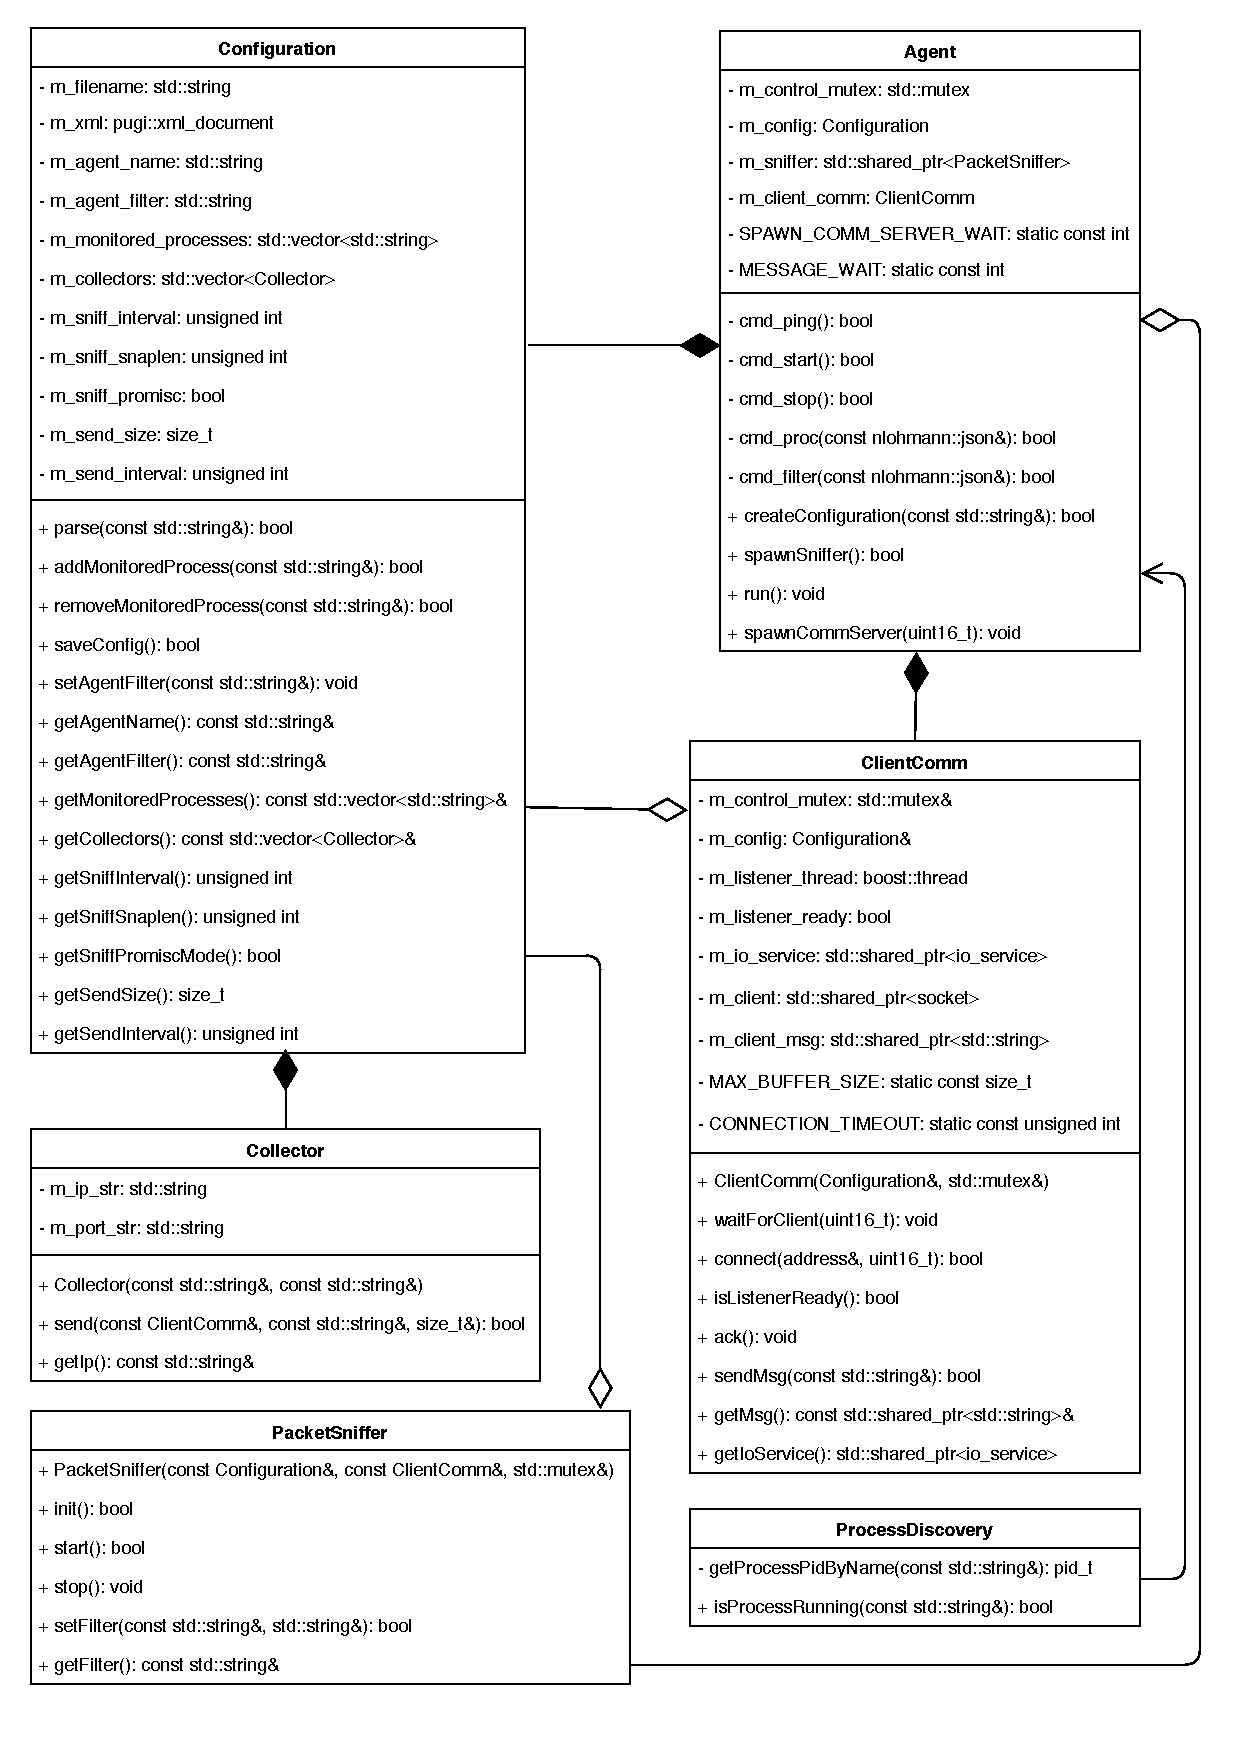
\includegraphics[scale=0.85]{agent.pdf}
	%	\caption{Dátový diagram}
\end{figure}

\textbf{ProcessDiscovery} \\

Slúži na zistenie stavu procesu. Rôzna implementácia pre Windows aj Linux, keďže zisťovanie informácií o procesoch je platformovo závislá záležitosť. Používa sa funkcia \textit{isProcessRunning}, ktorej vstupom je názov procesu. Vracia sa bool hodnota podľa toho, či daný proces beží alebo nie. Implementácia na Windowse využíva Windows API, pomocou ktorej sa iteruje cez bežiace procesy a porovnáva sa názov exekuovateľného súboru s tým, ktorý hľadáme. \\

Na Linuxe sme pridali funkciu \textit{getProcessPidByName}, ktorej vstupom je názov procesu a vracia pid príslušného procesu alebo -1, ak sa daný proces nenašiel. Vyhľadávanie pidu sa deje pomocou prechádzania adresára \textit{/proc/}. Samotná funkcia \textit{isProcessRunning} v tomto prípade kontroluje, či funkcia \textit{getProcessPidByName} vrátila valídny pid a následne sa zavolá systémová operácia \textit{kill} so signálom 0 (prázdny signál) a očakáva sa návratová hodnota 0 (to znamená, že daný proces beží a je možné nad ním zavolať \textit{kill}). \\

\textbf{Collector} \\

Slúži na odosielanie paketov na server. V konštruktore sa nastavuje \textit{ip adresa} a \textit{port}. Funkcia \textit{send} dostáva na vstup inštanciu triedy \textit{ClientComm}, dáta (string) a premennú typu \textit{size\_t}, do ktorej sa uloží počet odoslaných bajtov. Vracia sa bool hodnota podľa úspechu alebo neúspechu odosielania. Mechanizmus odosielania je nasledovný – nadviaže sa spojenie, odošle sa číslo (štyri bajty), ktoré reprezentujú, koľko dát sa má odoslať a nakoniec sa odošlú samotné dáta. \\

\noindent V main funkcii:
\begin{itemize} 
	\item vytvorí sa objekt Agent
	\item vytvorí sa konfigurácia (createConfiguration)
	\item Agent zavolá spawnSniffer – inicializácia odchytávania paketov
	\item vytvorí sa komunikačný server na porte 8888 (spawnCommServer)
	\item zavolá sa run \\
\end{itemize}

\textbf{Configuration} \\

Uchováva a menežuje konfiguráciu agenta. Okrem metód na vyžiadanie jednotlivých parametrov (get), obsahuje metódu na parsovanie konfiguračného súboru z disku pod názvom \textit{parse}, kde vstupom je názov súboru a vracia sa hodnota bool podľa úspešnosti operácie. Ďalej obsahuje metódy na pridanie (\textit{addMonitoredProcess}), mazanie (\textit{removeMonitoredProcess}) procesov, nastavovanie filtra (\textit{setAgentFilter}) a na ukladanie konfigurácie (\textit{saveConfig}). \\

\textbf{ClientComm} \\

Riadi komunikáciu s Monitorom (postarom Client). Konštruktor nastavuje premenné konfigurácie, mutex a vytvorí sa shared\_ptr z io\_service. Funkcia waitForClient čaká na spojenie s Monitorom. Vstupným argumentom je port, na ktorom sa má počúvať. waitForClient vytvorí UDP server na porte a čaká na pripojenie (maximálne jedno), potom sa vypne. Spojenie sa vytvorí až po identifikačnom „handshake“ (podanie rúk), ktorý obsahuje reťazec „agentSearch“. Connect slúži na inicializáciu TCP spojenia po handshake. Číslo portu je odosielané tou stranou, ktorá inicializuje spojenie (správa v tvare agentSearch/<port>). V prípade prijatia správy “agentSearch/<port>” na agentovi, daný agent sa pripojí na port a odošle správu “agentName/<meno agenta>”. Funkcia sendMsg slúži na odosielanie správy, ktorú dostáva na vstup. 
 \\

\textbf{PacketSniffer} \\

Trieda, ktorá slúži na odchytávanie sieťových paketov. Pri konštrukcií sa nastaví premenná typu Configuration, ClientComm a mutex. Funkcia init slúži na vypísanie všetkých dostupných zariadení na odchytávanie paketov a nechá užívateľa vybrať, na ktorom sa bude odchytávať. Tento mechanizmus je existuje, pretože sa stáva, že na niektorých počítačoch je prítomných viacero zariadení na odchytávanie a v prípade automatického výberu zariadenia by sa nemuselo vybrať správne. Funkcia start naštartuje odchytávanie v novom vlákne.

Toto vlákno najprv inicializuje odchytávacie zariadenie funkciou \textit{pcap\_open\_live}, do ktorej vstupujú parametre ako: názov zariadenia, snapshot length, promiscuous mode, read timeout, z čoho všetky až na názov zariadenie vieme zmeniť v konfiguračnom súbore - elementy začínajúce Sniff. Samotné pakety sú odchytávané funkciou \textit{pcap\_next\_ex} v cykle. Táto funkcia vracia smerník na dáta paketu a jeho veľkosť. Paket posunieme metóde \textit{handlePacket}, ktorá na základe štruktúr v súbore \textit{netdefs.h} sparsuje daný paket a vráti o aký protokol sa jedná, zdrojovú a cieľovú IP adresu, zdrojový a cieľový port a čas kedy bol paket zachytený. Tieto dáta sú posunuté metóde \textit{writePacket}, ktorá ich transformuje do formátu, ktorý príjime serverový komponent \textit{HBaseWriter} a zapíše ich do databázy. To, či vlákno beží alebo nie je určené členskou premennou \textit{m\_run\_thread}, ktorá je pri požiadavke na zastavenie agenta nastavená na false. \\

Manipulovať s filtrom vieme metódami \textit{getFilter} a \textit{setFilter}. \textit{setFilter} vie aj za behu agenta nastaviť filter a vrátiť chybovú správu, ak sa to nepodarí. V prípade neúspechu je táto chybová správa poslaná monitoru a informuje tak použivateľa. \\

Formát, v akom sa posielajú pakety je rovnaký ako v predošlom riešení tímového projektu: \\

\noindent <timestamp> \\
<protokol> \\
<zdrojova\_ip> \\
<cielova\_ip> \\
<zdrojovy\_port> \\
<cielovy\_port> \\
<data\_paketu\_hexstring> \\

Pakety sú oddelené značkou “End of packet” a koniec paketov je označený ako “End of packets file”. Tento formát nie je ideálny, pretože veľkosť každého posielaného paketu je 2x väčšia ako keby sa posiela v binárnej podobe. Možné riešenie tohto problému sme navrhli v kapitole \textit{Pohľad do budúcnosti}. \\


\textbf{Agent} \\

Metóda \textit{createConfiguration} berie ako vstupný parameter názov súboru .xml s konfiguráciami agenta. Tieto konfigurácie pošle ďalej triede Configuration, ktorá si ich rozparsuje a uloží. \textit{spawnSniffer} inicializuje objekt PacketSniffer a tým odchytávanie paketov. Táto inicializácia sa deje len raz za beh programu. \textit{spawnCommServer} berie na vstupe číslo portu. Vnútri tejto metódy sa vytvorí vlákno, v ktorom sa v nekonečnom cykle každých 1000 milisekúnd komunikuje prostredníctvom ClientComm s Monitorom. Toto vlákno sa odpojí (detach) a ostáva žiť do konca programu (alebo do systémového prerušenia/nezachytenej chyby). Vo funkcii \textit{run} sa spracúvajú v nekonečnej slučke každých 100 milisekúnd správy z triedy ClientComm. Z príchodzej json správy sa vyparsuje informácia o príkaze a ten sa následne spustí. Momentálne sa podporujú príkazy na overenie pripojenia (ping), vypnutie (stop) a zapnutie (start) sniffera, nastavenie a vypísanie filtra počas behu (filter get/filter set) a správu sledovania procesov (pridávanie, mazanie, získanie stavu - proc add / proc del / proc get). Viac o formáte, v akom sú príkazy prijímané tu: \\

\begin{figure}[h!]
	\centering
	\label{graf1}
	\includegraphics[scale=0.75]{graf2.jpg}
	\caption{Vylepšenie výkonnosti agenta po aplikovaných zmenách}
\end{figure}

\subsection{Konfigurácia}

Tvar: \\ 
\begin{lstlisting}
<Configuration> 
	<Sender> 
		<BufferSize>128000</BufferSize> 
		<Interval>10</Interval> 
		<Collector>ip:port</Collector> 
	</Sender> 
	<Agent> 
		<Name>AgentA</Name> 
		<Filter>tcp or udp</Filter> 
		<MonitoredProcesses> 
			<Process>hello.exe</Process> 
			<Process>world.exe</Process> 
		</MonitoredProcesses> 
		<SniffInterval>1000</SniffInterval> 
		<SniffSnapLen>2048</SniffSnapLen> 
		<SniffPromiscMode>false</SniffPromiscMode> 
	</Agent> 
</Configuration> 
\end{lstlisting}

V konfigurácií agenta máme dva základné komponenty a to \textit{Sender} – nastavenie odosielania na kolektor paketov a \textit{Agent} – nastavenia špecifické agentovi a jeho funkcií.
V Sender nastaveniach sa určuje \textit{BufferSize}, ako meno naznačuje ide o veľkosť buffera (v bajtoch), do ktorého sa vkladajú pakety. \textit{Interval} udáva počet sekúnd, po ktorých prebehne replikácia. Element \textit{Collector} obsahuje adresu a port, na ktorú sa má agent pripájať a pakety odosielať. \\

Agent má nastavenia \textit{Name}, ktoré udáva meno agenta. \textit{Filter} nastavuje filtrovanie paketov. Do \textit{MonitoredProcesses} máme možnosť zadávať procesy, ktoré chceme monitorovať (pre tvar zadávania viď príklad tvaru). \textit{SniffInterval} udáva interval (v milisekundách), v ktorom sa odchytávajú pakety. \textit{SniffSnapLen} určuje aká časť paketu sa má odchytiť (v bajtoch). \textit{SniffPromiscMode} popisuje, stav promiskuitného módu (zapnutý/vypnutý – true/false). \\

\begin{figure}[h!]
	\centering
	\label{graf1}
	\includegraphics[scale=0.75]{uk1.jpg}
	\caption{Ukážka spustenia agenta na Windowse}
\end{figure}

\begin{figure}[h!]
	\centering
	\label{graf1}
	\includegraphics[scale=0.75]{uk2.jpg}
	\caption{Ukážka spustenia agenta na Linuxe}
\end{figure}

\section{Zmeny klienta}

Tento komponent sme premenovali na Monitor, pretože Client je veľmi mätúci názov a neodráža to, čo sa pomocou tohto nástroja vykonáva. \\

\noindent Zmenila sa taktiež štruktúra projektu, ktorá vyzerá momentálne nasledovne:
\begin{itemize} 
	\item Client: projektové súbory Visual Studia (.sln, .vxcproj, ...) 
	\item src: zdrojové kódy - .hpp aj .cpp 
	\item CMakeLists.txt – cmake pre kompiláciu na Linuxe 
	\item Readme.md – informácie o projekte 
	\item config\_monitor.xml - konfigurácia monitoru\\
\end{itemize}

\noindent Prehľad rozsiahlych zmien a novej funkcionality:
\begin{itemize} 
	\item pripojenie na Mysql databázu
	\item obojsmerná komunikácia s agentmi (predtým iba monitor -> agent)
	\item zavedený komunikačný formát JSON (predtým obyčajný text)
	\item pridaný príkaz "discover" na vyhľadanie agentov v sieti (predtým sa tento proces dial len pri spustení programu)
	\item pridaný príkaz "list", ktorý vypíše pripojených agentov, skontroluje ich stav and aktualizuje ho v databáze
	\item pridaný príkaz "filter get“, ktorý vypíše nastavenia filtra na konkrétnom agentovi
	\item príkaz "filter set" informuje používateľa, či sa daný filter podarilo aplikovať
	\item nový príkaz "proc" na vyžiadanie stavu, pridanie alebo odobratie monitorovaných procesov (get vyžiada stav - môže byť running(bežiaci)/not running(nebežiaci)) 
	\item stavy agentov a monitorované procesy sú periodicky aktualizované v databáze \\
\end{itemize}

\begin{figure}[h!]
	\centering
	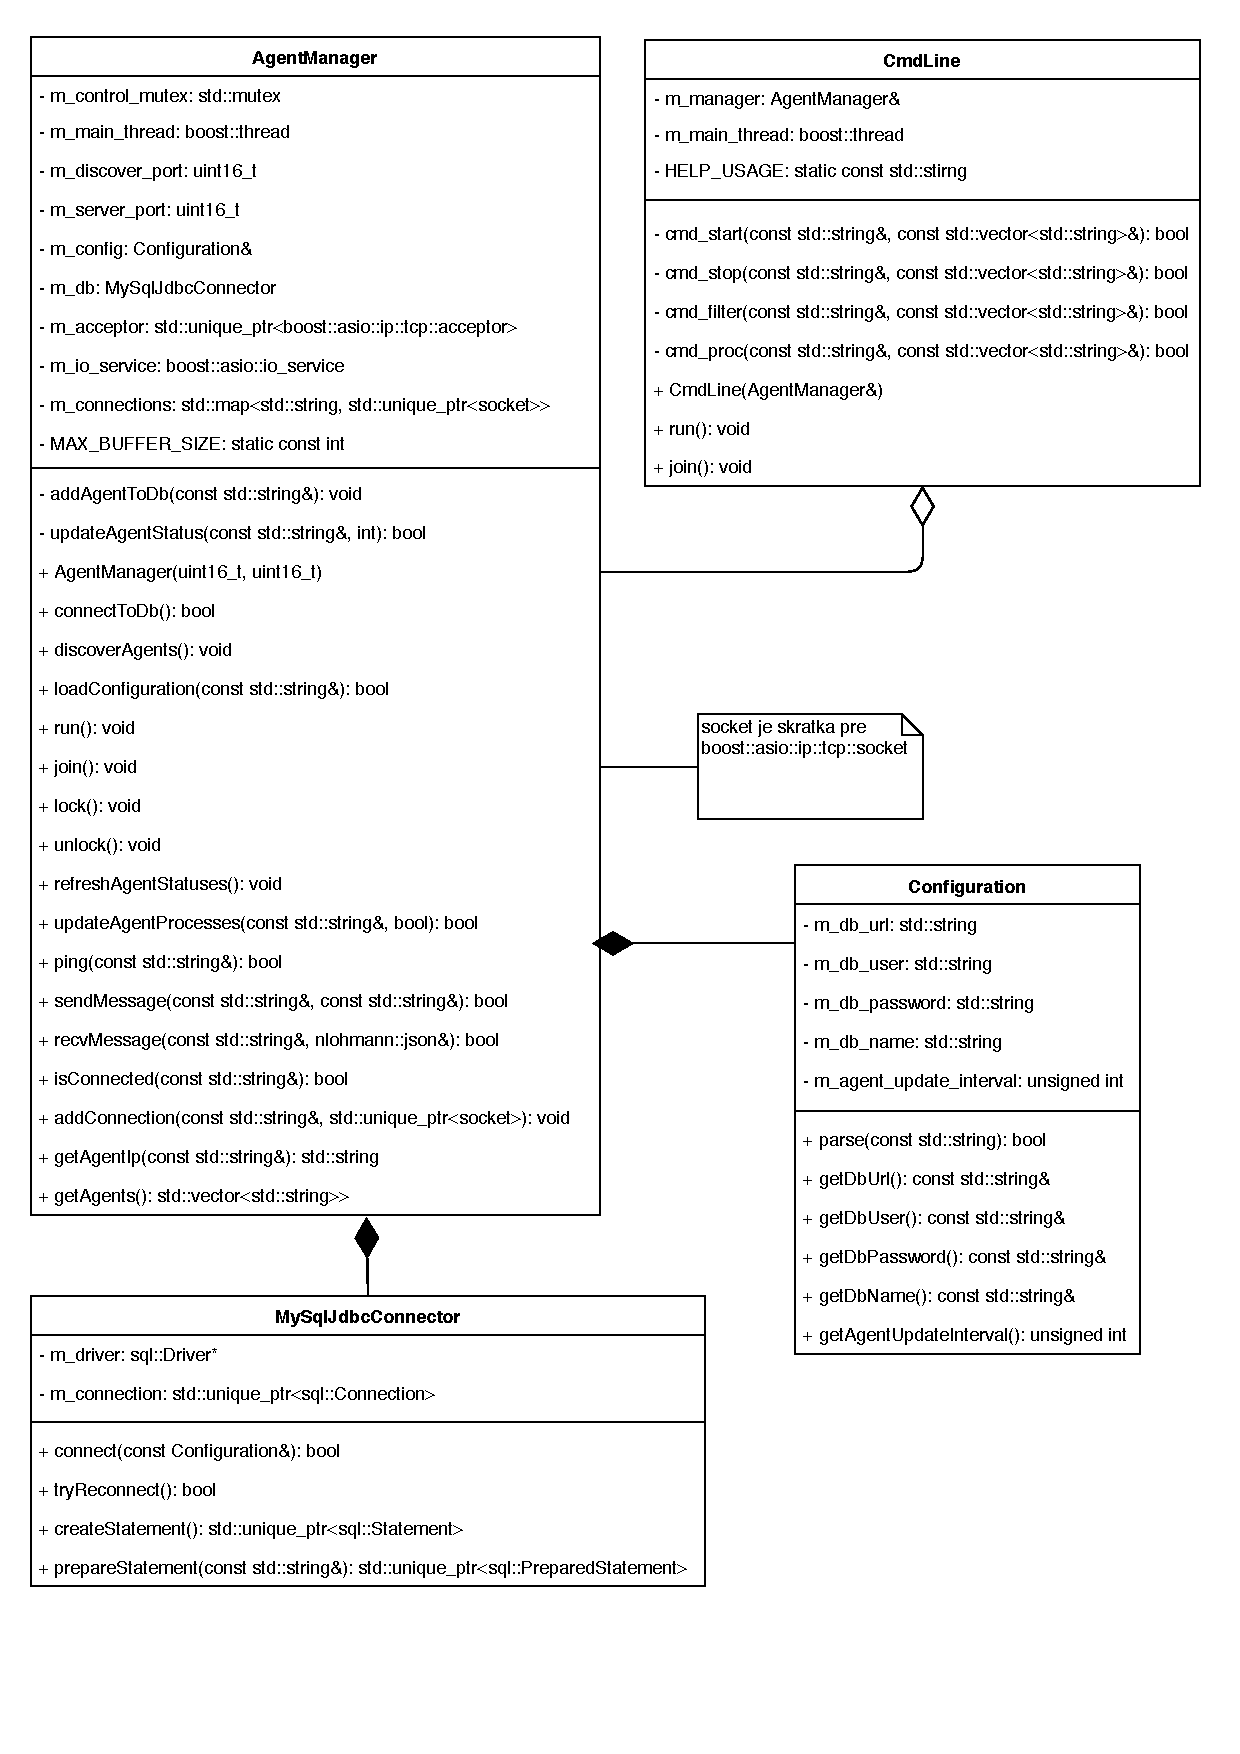
\includegraphics[scale=0.75]{monitor.pdf}
\end{figure}

\textbf{AgentManager} \\

Ako názov naznačuje, táto trieda slúži na menežment, čiže riadenie agentov v sieti. Boli do nej zakomponované komponenty, ktoré sa nachádzali v projekte ako samostatné triedy. \\

AgentManager má v sebe inštanciu objektu \textit{Configuration}, ktorá udržiava konfigurácie načítané z .xml súboru, inštanciu objektu \textit{MySqlJdbcConnector} pre prístup do databázy a mapovanie názvov agentov na konekcie k nim. \\

Pri vytváraní objektu sa v konštruktore nastaví inštancia konektora na databázu a dva porty (jeden pre odosielanie dát ohľadom procesov, ktorých stav sa po novom monitoruje a ďalší, serverový port). \\

Jednou z nových funkcionalít je aj pridanie konfigurácie (podobne ako v projekte Agent) a jej načítanie pomocou funkcie \textit{loadConfiguration}, ktorá ako vstupný parameter berie relatívnu cestu k .xml súboru s konfiguráciou a vracia hodnotu true/false podľa toho, či sa daná konfigurácia načítala správne alebo nie. \\

Na pripojenie sa k databáze sa využíva funkcia \textit{connectToDb}, ktorá je v podstate iba premostením funkcie triedy \textit{MySqlJdbcConnector}, ale zároveň kontroluje, či pripojenie prebehlo úspešne a podľa toho vracia pravdivostnú hodnotu. Na vkladanie do databázy sa používa \textit{prepared statement}, ktorý je rýchlejší než klasický statement a taktiež zamedzuje SQL injection, keďže vstupné hodnoty sa vkladajú namiesto zástupcov a taktiež sa korektne spracúvaju špeciálne znaky. \\

Funkcia \textit{discoverAgents} slúži na vyhľadanie agentov v sieti, presnejšie odošle UDP broadcast, na ktorý agenti neskôr reagujú. \\

Celý proces sieťovej komunikácie sa spúšta až funkciou \textit{run}. V tejto funkcií sa inicializuje \textit{acceptor} na tvorbu spojení, inicializuje sa hlavné vlákno (\textit{m\_main\_thread}), v ktorom beží v nekonečnej slučke počúvanie na pokus o vytvorenie nového spojenia s agentom. Po vytvorení úspešného spojenia sa spojenie pridá do mapovania spojení a aktualizuje sa časový údaj o spojení v databáze. Ako ďalšie sa spúšťa vlákno, ktoré udržiava spojenie s databázou a aktualizuje stavy agentov a sledovaných procesov. Nad týmto vláknom sa volá metóda \textit{detach}, keďže chceme, aby vlákno pracovalo na pozadí až do terminácie programu. \\

Na možnosť obojsmernej komunikácie s agentmi sa pridala k funkcií na odosielanie \textit{sendMessage} funkcia na príjmanie \textit{recvMessage}. \\

\textbf{Configuration} \\

Má za úlohu načítať a udržať stav konfigurácie pre \textit{Monitor}. Na načítavanie slúži funkcia \textit{parse}, ktorá ako vstup dostáva relatívnu cestu k .xml súboru. Načíta jednotlivé hodnoty z konfigurácie a vráti true ak všetko prebehlo v poriadku, inak false. Ďalej sa v tejto triede nachádzajú get metódy pre všetky definované konfigurácie. \\

\textbf{MySqlJdbcConnector} \\

Slúži ako spojka medzi monitorom a databázou. Udržiava v sebe pointer na driver a konekciu. Funkcia \textit{connect} so vstupným parametrom triedy \textit{Configuration} má za úlohu pripojenie na databázu, pričom prístupové údaje, sieťovú adresu a meno databázy berie z konfigurácie. Podľa úspešnosti pripojenia vracia bool. Bolo potrebné vytvoriť aj funkciu \textit{tryReconnect}, ktorá overí, či spojenie stále existuje a ak neexistuje, pokúsi sa pripojiť znova. Potreba vychádzala z faktu, že po určitej dobe sa pripojenie zhadzovalo. Na vytváranie SQL príkazov sa používajú funkcie \textit{createStatement} a \textit{prepareStatement}, ktoré vracajú unikátny pointer na daný typ výroku. \\

\textbf{CmdLine} \\

Pri konštrukcií je potrebné posunúť ako argument \textit{AgentManager}, ktorého referencia sa uloží. Funkcionalita \textit{CmdLine} sa spúšta pomocou metódy \textit{run}, ktorá spustí hlavné vlákno, ktoré beží v nekonečnej slučke, spracúva zadané príkazy a deleguje funkcionalitu na príslušné funkcie podľa zadaných príkazov. Dostupné príkazy umožňujú spustiť a zastaviť odchytávanie paketov, nastavenie alebo získanie aktuálneho nastavenia filtra, výpis stavu sledovaných procesov, pridanie alebo mazanie sledovaného procesu. \\

\noindent V main funkcií Monitora prebiehajú nasledujúce kroky:
\begin{itemize} 
	\item vytvorenie objektu AgentManager, discover port sa nastavuje na 8888 a server port na 9999
	\item manager zavolá načítanie konfigurácie
	\item manager sa pripojí na databázu
	\item manager zavolá funkciu discoverAgents
	\item zavolá sa run
	\item vytvorí sa objekt CmdLine
	\item zavolá sa run
	\item na konci prebieha synchronizácia vláken z oboch objektov \\
\end{itemize}

\noindent Dostupné príkazy a ich syntax:

\noindent \textit{Help: \\
discover -> discover agents on network \\
list -> list of all connected agents (checks if alive) \\
stop <agent> -> stop agent \\
start <agent> -> start agent \\
filter <agent> get|set <filter> -> get/set filter on agent \\
proc <agent> get|add <process>|del <process> -> manipulate monitored processes on agent} \\

\subsection{Konfigurácia}

Tvar: \\ 

\begin{lstlisting}
<Configuration> 
	<MysqlDatabase> 
		<Url>tcp://host:port</Url> 
		<User>user</User> 
		<Password>password</Password> 
		<Name>database\_name</Name> 
	</MysqlDatabase> 
	<UpdateInterval>10</UpdateInterval> <!-- Seconds --> 
</Configuration> 
\end{lstlisting}

Element \textit{MysqlDatabase} obsahuje údaje potrebné na pripojenie sa k MySQL databáze a prepnutie sa na konkrétnu databázu. Na pripojenie sa je potrebná adresa (element Url), používateľ v databáze (User), používateľské heslo (Password) a názov schémy respektíve databázy (Name). Element \textit{UpdateInterval} udáva počet sekúnd, po ktorých sa vyžiada stav agentov z monitora. \\
\newpage

\section{Komunikácia medzi agentom a monitorom}
Je v princípe obojsmerná, ale efektívne agent len odpovedá na požiadavky monitoru. Formát komunikácie je JSON. Agent príjme požiadavku a v určitých prípadoch pošle naspäť odpoveď. Na parsovanie JSON používame “knižnicu” nlohmann.

\subsection{Monitor -> agent}

Formát požiadavky, ktorú vie poslať monitor na agenta:

\begin{lstlisting}
{
	“cmd”: <string>,
	“action”: <string>,
	“data”: <variable> 
}

\end{lstlisting}

Kľúč \textit{cmd} môže byť: ping, start, stop, filter, proc. Kľúč \textit{action} závisí od \textit{cmd} a \textit{data} od \textit{action}.

\begin{table}[h!]
	\centering
	\begin{tabular}{|c|c|c|c|}
		\hline
		\textbf{cmd} & \textbf{action} & \textbf{data} & \textbf{Popis}  \\
		\hline
		ping & - & - & Zistí či je agent online. \\
		\hline
		start & - & - & Zapne sniffer na agentovi.  \\
		\hline
		stop & - & - & Zapne sniffer na agentovi.  \\
		\hline
		filter & get, set & get: -,set: <string> & Získa/nastaví filter \\
		& & & na agentovi.  \\
		\hline
		proc &  get, add, del & get: -, add: <string>, & Získa/pridá/zmaže \\
		& &  del: <string> &  monitorovaný\\
		& & & proces na agentovi. \\ 
		\hline
		
	\end{tabular}
	\label{Tab:1}
\end{table}

\noindent Príklad takejto požiadavky na agenta:

\begin{lstlisting}
{
	“cmd”: “filter”, 
	“action”: “set”, 
	“data”: “tcp port 80” 
}
\end{lstlisting}


\subsection{Agent -> monitor}
\begin{lstlisting}
{
	“response”: <variable> 
}
\end{lstlisting}


Odpoveď agenta na požiadavku od monitoru je veľmi jednoduchá, pretože agent vždy len odpovedá, teda monitor pozná kontext danej odpovede. Príklad odpovede (pri úspešnej zmene filtra) na požiadavku na zmenenie filtra uvedenú vyššie:

\begin{lstlisting}
{
	“response”: “ok” 
}
\end{lstlisting}


\begin{table}[h!]
	\centering
	\begin{tabular}{|c|c|}
		\hline
		\textbf{Odpoveď na} & \textbf{response}  \\
		\hline
		ping & ``pong'' \\
		\hline
		start & - \\
		\hline
		stop & - \\
		\hline
		filter set &  ``ok''/chybová správa   \\
		\hline
		filter get &  aktuálne nastavený filter v snifferi   \\
		\hline
		proc add &  ``ok''/``no'' \\
		\hline
		proc del &  ``ok''/``no'' \\
		\hline
		proc get &  {“proces”: <0|1>, “proces2”: <0|1>, ..} alebo \{\} \\
		\hline
		
	\end{tabular}
	\label{Tab:1}
\end{table}

\section{Zmeny HBaseWriter} 
HBaseWriter je hlavná časť serveru, ktorá prijíma pakety od agentov. Pretože sa trochu menil formát, v akom agent posiela pakety, jeho parsovanie sa muselo zmeniť aj tu. Predošlý agent zapisoval pakety na poslanie do súboru, potom vytvoril Java proces \textit{HBaseSender} (túto časť už nepoužívame), ktorý tento súbor prečítal a následne odoslal jeho obsah do \textit{HBaseWriter} na server. \\
	
Keďže náš agent už posiela pakety z pamäte a nie zo súboru, museli sme odstrániť \textit{carriage return} (\r znak) z parsovania v \textit{HBaseWriter}. Stretli sme sa s ďalším problémom, kde predošlý \textit{HBaseSender} posielal obsah prečítaného súboru cez \textit{DataOutputStream} v Jave a \textit{HBaseWriter} ho prijímal cez \textit{DataInputStream}. Tento spôsob garantoval, že sa pakety od agenta príjmu naraz. No keďže náš agent posiela pakety cez \textit{boost tcp socket}, nie je garantované, že prídu naraz, na čo bol \textit{HBaseWriter} stavaný. Preto, keď agent ide poslať pakety, najprv pošle 4 bajty (integer), ktoré reprezentujú veľkosť dát, ktoré ide poslať, aby \textit{HBaseWriter} vedel koľko bajtov má čítať. Toto môžeme vidieť v nasledujúcom kóde:

 %KOOOOOOOOOOOOOOOOOOOOOOOD
 
 
\noindent Okrem spomenutých problémov sme v HBaseWriter nič na funkcionalite nemenili, no boli trochu upravené správy, ktoré sa vypisujú na obrazovku. \\
 
\section{Zmeny v detektoroch}
Oproti predošlému TP sa v detektoroch funkčne veľa nezmenilo, no opravili sme chyby v parsovaní paketov, kde aj napriek importovaniu knižnice, ktorá to mala vykonávať (\textit{jnetpcap}), táto knižnica nebola správne použitá. Podobne sme si všimli, že detektory parsovali paket až od IP hlavičky. \\

Do oboch detektorov (\textit{TCPDetection} a \textit{UDPDetection}) bolo taktiež pridané spojenie s MySQL databázou, keď prijde k detekcii. Na prácu s MySQL používame JDBC API. Do Maven projektového súboru (\textit{pom.xml}) bolo treba pridať:

\begin{lstlisting}
<dependency>
	<groupId>org.mariadb.jdbc</groupId>
	<artifactId>mariadb-java-client</artifactId>
	<version>1.7.4</version>
</dependency>
\end{lstlisting}

Používame mariadb klienta verziu 1.7.4, pretože na serveri je použitá JRE (Java Runtime Environment) verzia 7 a vyššie verzie mariadb klienta ako 1.7.4 sú kompatibilné len s JRE 8. \\

Jedna z dalších zmien bola upgrade \textit{jnetpcap} knižnice na verziu 1.4.r1425-1g v \textit{pom.xml} daného detektoru. Museli sme stiahnuť zdieľané knižnice \textit{jnetpcap}, ktoré sú kompatibilné s 1.4 verziou, pretože na serveri boli použité pre verziu 1.3. Všetky dôležité zdieľané knižnice, ktore sú dôležité na chod \textit{jnetpcap} sme nakopírovali do \textit{/usr/lib}, teda detektory už nemusia byť spúšťané s parametrom \textit{-Djava.library.path=/usr/local/sbin}. \\

Oba detektory sú spúšťané so zoznamom IP adries, ktoré majú monitorovať pri parsovaní paketov. \\

Na skompilovanie detektoru treba vojsť do jeho koreňového priečinku a spustiť nasledovné príkazy: \\

\noindent \textit{mvn clean \\
mvn compile \\
mvn package} \\

Pri úspešnej kompilácii sa v priečinku target vytvorí .jar súbor, ktorý môžeme spustiť. \\

\noindent \textit{TCPDetection} \\

Nachádza sa na serveri v priečinku \textit{/home/timak2016/TCPDetection} a .jar súbor sa nachádza v priečinku \textit{target}. \\

\noindent \textit{java -jar TCPDetectionModule-0.1.0.jar 147.175.106.17} \\

Keď sa vo fronte \textit{PCAPS\_TCP} nachádza .pcap súbor z floodovania, jeho detekcia vyzerá nasledovne: \\

\noindent [TCPDetection] Starting detector on 01152019170142.pcap336636293622419282.tmp \\
>> Parsed /tmp/01152019170142.pcap336636293622419282.tmp (packets: 996, monitored: 657) \\
>> SYN count: 338, FIN count: 1 \\
Value 653, Threshold: 200 \\
$[+]$ TCP flood alert for destination: 147.175.106.16\_80, value: 653 \\

Výsledky detekcie sa zapisujú do databázy do tabuľky \textit{tcp\_flood}. Je do nej zapísaná IP adresa a port, na ktorej sme detegovali flood spolu s časom kedy. \\

\noindent \textit{UDPDetection} \\

Nachádza sa na serveri v priečinku /\textit{home/timak2016/UDPDetection} a .jar súbor sa nachádza v priečinku \textit{target}. Detektor vieme spustiť nasledovným spôsobom: \\

\noindent \textit{java -jar UDPDetectionModule-0.1.0.jar 147.175.106.17} \\

Keď sa vo fronte \textit{PCAPS\_UDP} nachádza .pcap súbor z floodovania, jeho detekcia vyzerá takto (výstup z UDP detektoru): \\

\noindent [UDPDetection] Starting detector on 01202019152611.pcap8199263204614265330.tmp \\
>> Parsed /tmp/01202019152611.pcap8199263204614265330.tmp (packets: 4505, monitored: 4505) \\
From destination: 0, to destination: 4505 \\
>> Ratio: 4505.0, MAX\_RATIO: 300.0 \\
$[+]$ UDP flood alert to 147.175.106.17 from 147.175.106.16 \\

Výsledky detekcie sa zapisujú do databázy do tabuľky \textit{udp\_flood}. Sú do nej zapísané cieľová a zdrojová IP adresa s časom kedy. \\
\newpage

\section{Databáza}
Ako databázu sme použili MySQL, ktorá beží na serveri. Databázu tvoria 4 tabuľky: agents, processes, tcp\_flood a udp\_flood. Vo väčšine tabuliek používame stĺpec pre IP adresu, ktorej typ je varchar(15). Toto je z dôvodu jednoduchosti a uvedomujeme si, že to mohol byť dátový typ integer a manipulácia s ním mohla byť pomocou MySQL funkcii INET\_ATON() a INET\_NTOA(). \\

\textbf{agents} \\

Táto tabuľka je napĺňaná z monitoru. Reprezentuje všetkých agentov, ktorí kedy boli monitorovaní. Status agentov je sprevádzaný časom, kedy bol status obnovený. Keďže status agenta je možné zmeniť len prostredníctvom monitoru (t.j. ak je monitor pripojený na agenta, status agenta je periodicky obnovovaný a pri jeho zmene sa zmení status a čas v databáze). \\

Agent je do tabuľky vložený, keď monitor nadviaže spojenie s agentom. Agenti z tabuľky nie sú mazaní. \\

Jej schéma je nasledovná: \\

\noindent id: int \\
name: varchar(255) \\
ip: varchar(15) \\
status: tinyint \\
last\_updated: timestamp \\

\textbf{processes} \\

Taktiež napĺňaná z monitoru. Reprezentuje všetky monitorované procesy na všetkých agentoch. Jej schéma je nasledovná: \\

\noindent id: int \\
agent\_id: int \\
name: varchar(255) \\
monitored: tinyint \\
status: tinyint \\

Princíp fungovania je nasledovný: keď sa pridá nový monitorovaný proces do zoznamu agentovi, je vložený do databázy a jeho počiatočné hodnoty sú \textit{monitored} = 1 a status je určený podľa toho či reálne beží na agentovi. Keď sa proces zo zoznamu monitorovaných procesov na agentovi zmaže, v databáze je zmenená hodnota \textit{monitored} na 0. Každý proces v tejto tabuľke je viazaný na agenta podľa jeho id v tabuľke \textit{agents}. \\

\textbf{tcp\_flood} \\

Do tabuľky sa zapisuje len keď je TISMA systémom zistený TCP flooding na analyzovaných paketoch. \\

\noindent id: int \\
ip: varchar(15) \\
port: int \\
value: int \\
timestamp: timestamp \\

\textbf{udp\_flood} \\

Do tabuľky sa zapisuje len keď je TISMA systémom zistený UDP flooding na analyzovaných paketoch. \\

\noindent id: int \\
source\_ip: varchar(15) \\
destination\_ip: varchar(15) \\
ratio: double \\
timestamp: timestamp \\
\newpage

\section{Web}
Jednou z častí zadania bolo vytvorenie web-stránky, ktorá bude vizualizovať stav, procesy a detekcie jednotlivých agentov. Celý web je vytvorený pomocou technológií PHP, HTML, CSS a JavaScript. Dáta sú vyberané z MySQL databázy a vrámci webu sú rozdelené do troch sekcií, opísaných nižšie. \\

\subsection{Agents}
V tejto sekcii je možné vidieť aktuálny stav jednotlivých agentov. A to konkrétne meno agenta, IP adresu agenta, jeho stav či beží alebo nie a čas kedy bol naposledy aktualizovaný status agenta. \\

\begin{figure}[h]
	\centering
	\includegraphics[scale=0.75]{agents.jpg}
	%	\caption{Dátový diagram}
\end{figure}

\subsection{Monitored Processes}
Tu je možné vidieť detailnejšie informácie o jednotlivých agentoch a to aké procesy sú kontrolované a či sú spustené na agentoch. \\

\begin{figure}[h]
	\centering
	\includegraphics[scale=0.75]{procs.jpg}
	%	\caption{Dátový diagram}
\end{figure}
Sú vypísané len procesy, ktoré majú v tabuľke hodnotu monitored 1 pre daného agenta. \\

\subsection{Detections}
V tejto časti sú zobrazené útoky. Konkrétne tu je možné pozorovať čas, kedy daný útok nastal a na ktorú IP adresu resp. agenta bol tento útok vykonaný. \\

\begin{figure}[h!]
	\centering
	\includegraphics[scale=0.75]{detections.jpg}
	%	\caption{Dátový diagram}
\end{figure}




\section{Build agentov}
Kompilácia agenta bola pozmenená, keďže sa pridali nové knižnice a zjednotil sa zdrojový kód pre obe platformy (Windows aj Linux). \\

Na Windowse je ku kompilácií potrebné Microsoft Visual Studio 2017 (v141).
Potrebné sú knižnice \textit{boost} (verzia 1.68.0), \textit{Npcap} a \textit{NPCAP SDK}. Je potrebné ich rozbaliť a nainštalovať (na ľubovoľné miesto na disku).  Pri knižnici \textit{Npcap} je potrebné zvoliť „Winpcap compact mode“. Ak už máme knižnice pripravené, pridáme do systémových premenných prostredia hodnoty: BOOST\_INCLUDE\_PATH, BOOST\_LIB\_PATH, NPCAP\_INCLUDE\_PATH, NPCAP\_LIB\_PATH a nastavíme ich tak, aby ukazovali na include alebo library cestu danej knižnice. \\

\noindent Príklad: \\
BOOST\_INCLUDE\_PATH=C:$\textbackslash$boost\_1\_68\_0\_32 \\
BOOST\_LIB\_PATH=C:$\textbackslash$boost\_1\_68\_0\_32$\textbackslash$lib32-msvc-14.1 \\
NPCAP\_INCLUDE\_PATH=C:$\textbackslash$npcap$\textbackslash$Include \\
NPCAP\_LIB\_PATH=C:$\textbackslash$npcap$\textbackslash$Lib \\
\\
Na kompilovanie treba pomocou Visual Studia otvoriť .sln súbor, ktorý sa nachádza medzi súbormi projektu. Vpravo máme okno „Solution Explorer“, v ktorom máme položku projektu („Agent“). V nastaveniach projektu je potrebné pridať knižnice, ktoré využívame. Navigujeme:
\textit{Right-click „Agent“ $\rightarrow$ Properties $\rightarrow$ Configuration Properties~$\rightarrow$ VC++ Directories}.
Predtým než začneme pridávať nastavenia, je potrebné sa uistiť, že máme v hornej lište nastavené políčko “Configuration” na “All Configurations” a “Platform” na “Win32”. Pridáme do tabuľky „General“ v riadku pre „Include directories“ cesty pre include našich knižníc - \$(BOOST\_INCLUDE\_PATH);\$(NPCAP\_INCLUDE\_PATH);  a do „Library directories“ \$(BOOST\_LIB\_PATH);\$(NPCAP\_LIB\_PATH);. \\

Na Linuxe je potrebný kompilátor \textit{gcc} (verzia 5.1 a vyššie). Rovnako ako pri Windowse nainštalujeme knižnice \textit{boost} (ľubovoľný spôsob inštalácie) a \textit{libpc.p} pomocou príkazu \textit{sudo apt-get install automake libpcap-dev build-essential}.
Ak sme \textit{boost} kompilovali sami, treba v súbore \textit{CMakeLists.txt} zmeniť set (BOOST\_ROOT "/home/user/boost\_1\_68\_0") tak, aby ukazoval na miesto, kde sme zdrojové súbory vykompilovali. Ak sme \textit{boost} nekompilovali sami, potom zmeníme v tom istom súbore hodnotu set (Boost\_NO\_SYSTEM\_PATHS TRUE) na FALSE.
\\

Po vykonaní všetkých týchto inštrukcií, stačí použiť príkazy „cmake .“ a následne „make“ v adresári so súborom \textit{CMakeLists.txt}, čím sa nám zdrojový kód skompiluje.
\\
\\
\textbf{CMake Agenta} \\
%-------------------- cmake treba naformatovat do kodoveho stylu
Pridané zdrojové súbory (zvlášť .hpp a .cpp) \\
file (GLOB CPP\_FILES src/*.cpp) \\
file (GLOB HPP\_FILES src/*.hpp) \\
\\
set (SOURCE\_FILES \$\{CPP\_FILES\} \$\{HPP\_FILES\}) \\
\\
Nastavenie libpcap symbolového súboru \\
\begin{lstlisting}
if (EXISTS /usr/lib/x86\_64-linux-gnu/libpcap.so) 
	set (LIBS /usr/lib/x86\_64-linux-gnu/libpcap.so) 
else () 
	set (LIBS /usr/lib/i386-linux-gnu/libpcap.so) 
endif ()
\end{lstlisting}

\\
Nastavenie boostu  \\
set (Boost\_USE\_STATIC\_LIBS OFF) \\
set (Boost\_USE\_MULTITHREADED ON) \\
set (Boost\_USE\_STATIC\_RUNTIME OFF) \\ \\
find\_package(Boost 1.68.0 COMPONENTS system filesystem chrono thread) \\ \\
Na konci sa naviažu zdrojové súbory \\
add\_executable(\$\{TARGET\_NAME\} \$\{SOURCE\_FILES\}) \\ \\
Nalinkujú sa knižnice  \\
target\_link\_libraries(\$\{TARGET\_NAME\} \$\{LIBS\} \$\{Boost\_LIBRARIES\}) \\ \\
A na záver sa nastaví kompilácia \\
target\_compile\_options(\$\{TARGET\_NAME\} PRIVATE -std=c++11) \\

\subsection{Build monitoru}
Potreba Microsoft Visual Studia (Windows), \textit{gcc} (Linux) a knižnice \textit{boost} (viď sekcia kompilácie Agenta) a navyše je potrebný MySQL Connector pre C++ (verzia 8.0). \\

Na Windowse vytvoríme pre cesty k include a library systémové premenné prostredia: MYSQL\_CONNECTOR\_INCLUDE\_PATH a MYSQL\_CONNECTOR\_LIB\_PATH. \\ \\
Príklad: \\
MYSQL\_CONNECTOR\_INCLUDE\_PATH=C:$\textbackslash$mysql-connector-c++-8.0.13-win32$\textbackslash$include \\
MYSQL\_CONNECTOR\_LIB\_PATH=C:$\textbackslash$mysql-connector-c++-8.0.13-win32$\textbackslash$lib$\textbackslash$vs14 \\ \\

Tieto hodnoty pridáme do nastavení projektu (podobne ako v časti pre Agenta) - \textit{Right-click project $\rightarrow$ Properties $\rightarrow$ Configuration Properties $\rightarrow$ VC++ Directories}, kde do „Include Directories“ pridáme \$(MYSQL\_CONNECTOR\_INCLUDE\_PATH); a do “Library directories” \$(MYSQL\_CONNECTOR\_LIB\_PATH);. Následne navigujeme od \textit{Configuration Properties $\rightarrow$ Linker $\rightarrow$ General} a do poľa „Additional Library Dependencies“ pridáme hodnotu \$(MYSQL\_CONNECTOR\_LIBRARY\_PATH);. Prepneme cez \textit{Linker $\rightarrow$ Input} a do “Additional Dependencies” pridáme názov knižnice~\textit{mysqlcppconn.lib}. \\ 

Na to, aby sme mohli program spúšťať, musíme do súboru s vygenerovaným .exe súborom ešte pridať knižnice \textit{mysqlcppconn-7-vs14.dll}, \textit{ssleay32.dll}, \textit{libeay32.dll} (z MySQL Connectora). \\

Na Linuxe je postup identický s postupom kompilácie Agenta, akurát je potrebné doinštalovať spomínaný Connector pre MySQL. \\
\textit{(Poznámka: Ak používame Debian, nesmie sa používať inštalácia z repozitára!).} \\
Kompiláciu stačí spustiť pomocou príkazov „cmake .“, potom „make“. \\ 

\textbf{CMake Monitoru} \\ \\
Veľmi podobná štruktúra ako pri Agentovi – rovnaké nastavenie \textit{boostu}, vyhľadávanie komponentov, až na symbolový súbor pre MySQL Connector.\\

\begin{lstlisting}
if (EXISTS /usr/lib/x86\_64-linux-gnu/libmysqlcppconn.so) 
	set (LIBS /usr/lib/x86\_64-linux-gnu/libmysqlcppconn.so) 
else () 
	set (LIBS /usr/lib/i386-linux-gnu/libmysqlcppconn.so) 
endif ()

\end{lstlisting}
\newpage

\section{Pohľad do budúcnosti}
\begin{itemize} 
	\item je vhodné začať sa zaoberať bezpečnosťou a integrovať ju do systému, kým nie je príliš veľký a rozmanitý
	\item pre začiatok by bola potreba, aby sa agenti autorizovali voči serveru (certifikáty, šifrovaná komunikácia) a aby webstránka mala SSL/TLS vrstvu (HTTPS protokol)
	\item PcapSender by mal ukladať posledne načítané ID paketu a neskôr ukladať od tohoto ID (ak je valídne) 
	\item zjednotenie serverových programov HBaseWriter, PcapSender, detekcie, do jedného java programu (pričom každý program by bol rôzny komponent programu)
	\item zlepšiť kvalitu behu programov za pomoci vlákien
	\item asynchrónna komunikácia medzi monitorom a agentom
	\item zmena formátu odosielaných paketov (ideálne na binárny) \\
\end{itemize}
\newpage

\section*{Záver}
\addcontentsline{toc}{section}{Záver}
Cieľom tohto tímového projektu bolo spevniť existujúce základy, ktoré vytvorili predošlé tímy. Toto sme dosiahli veľkými zmenami v jadre agenta a monitoru, ktoré nám umožnili zjednotiť zdrojový kód pre Windows aj Linux, použiť rovnakú knižnicu na zachytávanie sieťovej komunikácie, ktorá má rovnakú filter syntax apod. Použitie JSON v komunikácii medzi agentom a monitorom výrazne zjednoduší prácu pre budúce tímy, ak budú chcieť pridávať nové príkazy. Taktiež sme do infraštruktúry zakomponovali MySQL databázu, pomocou ktorej monitorujeme status agentov, bežiace procesy na nich a detegované útoky na agentov. V základnej konfigurácii sme dosiahli žiadne zaťaženie systému, na ktorom beží agent. \\
\newpage

\section*{Zoznam použitej literatúry}
\addcontentsline{toc}{section}{Zoznam použitej literatúry}

\newpage

\section*{Prílohy}
\pagenumbering{Roman}
\addcontentsline{toc}{section}{Prílohy}

\newpage
\end{document}
